\section{ueac.c File Reference}
\label{ueac_8c}\index{ueac.c@{ueac.c}}
{\tt \#include $<$stdio.h$>$}\par
{\tt \#include \char`\"{}ueac.h\char`\"{}}\par
{\tt \#include \char`\"{}ueaclib.h\char`\"{}}\par
{\tt \#include \char`\"{}cal\_\-table.h\char`\"{}}\par
{\tt \#include \char`\"{}filter.h\char`\"{}}\par
{\tt \#include \char`\"{}conversion.h\char`\"{}}\par
{\tt \#include \char`\"{}global.h\char`\"{}}\par
{\tt \#include \char`\"{}calibrate.h\char`\"{}}\par
{\tt \#include \char`\"{}lla.h\char`\"{}}\par


Include dependency graph for ueac.c:\begin{figure}[H]
\begin{center}
\leavevmode
\includegraphics[width=96pt]{ueac_8c__incl}
\end{center}
\end{figure}
\subsection*{Functions}
\begin{CompactItemize}
\item 
int {\bf lla\_\-input\_\-check} (char chan, {\bf ueac\_\-t} $\ast$system\_\-state)
\item 
void {\bf report\_\-instruction} ({\bf ueac\_\-t} $\ast$system\_\-state)
\item 
int {\bf ueac\_\-execute\_\-instruction} ({\bf ueac\_\-t} $\ast$system\_\-state)
\end{CompactItemize}
\subsection*{Variables}
\begin{CompactItemize}
\item 
{\bf lla\_\-data\_\-t} {\bf lla\_\-data}
\end{CompactItemize}


\subsection{Function Documentation}
\index{ueac.c@{ueac.c}!lla_input_check@{lla\_\-input\_\-check}}
\index{lla_input_check@{lla\_\-input\_\-check}!ueac.c@{ueac.c}}
\subsubsection{\setlength{\rightskip}{0pt plus 5cm}int lla\_\-input\_\-check (char {\em chan}, {\bf ueac\_\-t} $\ast$ {\em system\_\-state})}\label{ueac_8c_a1}




Definition at line 225 of file ueac.c.

References ueac::lla\_\-input.

Referenced by timer\_\-a0\_\-irq(), and ueac\_\-execute\_\-instruction().

\footnotesize\begin{verbatim}225                                                     {
226   int return_val=0;
227   if (system_state->lla_input&((unsigned long)(0x00000001<<chan))) {
228     return_val=1;
229   }
230   return (return_val);
231 }
\end{verbatim}\normalsize 


\index{ueac.c@{ueac.c}!report_instruction@{report\_\-instruction}}
\index{report_instruction@{report\_\-instruction}!ueac.c@{ueac.c}}
\subsubsection{\setlength{\rightskip}{0pt plus 5cm}void report\_\-instruction ({\bf ueac\_\-t} $\ast$ {\em system\_\-state})}\label{ueac_8c_a2}




Definition at line 233 of file ueac.c.

References ueac::instruction, ueac\_\-instruction::lla\_\-descriptor, ueac\_\-instruction::lla\_\-function, ueac\_\-instruction::lla\_\-period, ueac\_\-instruction::pin\_\-x, ueac\_\-instruction::pin\_\-x\_\-alt, ueac\_\-instruction::pin\_\-y, and ueac\_\-instruction::pin\_\-y\_\-alt.

\footnotesize\begin{verbatim}233                                               {
234   
235   printf("xin=%d ",system_state->instruction.pin_x);
236   printf("yin=%d ",system_state->instruction.pin_y);
237   printf("xout=%d ",system_state->instruction.pin_x_alt);
238   printf("yout=%d\n",system_state->instruction.pin_y_alt);
239   printf("descriptor=%d ",system_state->instruction.lla_descriptor);
240   printf("function=%d ",system_state->instruction.lla_function);
241   printf("period=%d\n",system_state->instruction.lla_period);
242 }
\end{verbatim}\normalsize 


\index{ueac.c@{ueac.c}!ueac_execute_instruction@{ueac\_\-execute\_\-instruction}}
\index{ueac_execute_instruction@{ueac\_\-execute\_\-instruction}!ueac.c@{ueac.c}}
\subsubsection{\setlength{\rightskip}{0pt plus 5cm}int ueac\_\-execute\_\-instruction ({\bf ueac\_\-t} $\ast$ {\em system\_\-state})}\label{ueac_8c_a3}




Definition at line 64 of file ueac.c.

References clear\_\-led\_\-screen(), ueac\_\-instruction::command\_\-reg, conversion\_\-result, convert\_\-a2d(), current\_\-output\_\-calibration(), ueacval::hundredth, I\_\-CONVERSION, lla\_\-data::input, ueac::instruction, ueac\_\-instruction::instruction\_\-type, ueacval::integer, led\_\-screen\_\-enable, lla\_\-add(), lla\_\-disable(), lla\_\-enable(), lla\_\-input\_\-check(), lla\_\-report(), lla\_\-data::output, ueac::pin\_\-current, pin\_\-data, ueac\_\-instruction::pin\_\-x, ueac\_\-instruction::pin\_\-y, system\_\-reset(), UEAC\_\-ALL\_\-I, UEAC\_\-ALL\_\-V, UEAC\_\-CAL, UEAC\_\-EXECUTE, UEAC\_\-LLA\_\-ADD, UEAC\_\-LLA\_\-DISABLE, UEAC\_\-LLA\_\-ENABLE, UEAC\_\-LLA\_\-REPORT, UEAC\_\-LOF, UEAC\_\-LON, UEAC\_\-READ\_\-I, UEAC\_\-READ\_\-V, UEAC\_\-READY, UEAC\_\-RST, ueac\_\-state, UEAC\_\-WRITE, V\_\-CONVERSION, ueac\_\-instruction::value, and write\_\-current().

Referenced by interpreter().

\footnotesize\begin{verbatim}64                                                    {
65   enum {OFF,ON};
66   int return_val=0;
67 
68 #ifndef LINUX
69   int i;
70   int probe_num;
71 #endif 
72   if (system_state->instruction.command_reg==UEAC_EXECUTE) {
73     switch (system_state->instruction.instruction_type) {
74     case UEAC_ALL_V:
75 #ifndef LINUX
76       for (i=0;i<25;i++) {
77         if (lla_input_check(i,system_state)) {
78           convert_a2d(I_CONVERSION,pin_data[i].filtered_result,&conversion_result,i);
79           printf("0.%03d,",conversion_result.integer);
80         }
81         else {
82           convert_a2d(V_CONVERSION,pin_data[i].filtered_result,&conversion_result,i);
83           printf("%d.%02d,",conversion_result.integer,conversion_result.hundredth);
84         }
85       }
86 #else 
87       printf("UEAC_ALL_V ");
88 #endif
89       break;
90     case UEAC_ALL_I:
91 #ifndef LINUX
92       for (i=0;i<25;i++) {
93         if (lla_input_check(i,system_state)) {
94           convert_a2d(I_CONVERSION,pin_data[i].filtered_result,&conversion_result,i);
95           printf("-%d,",conversion_result.integer);
96         }
97         else {
98           printf("%d,",system_state->pin_current[i]);
99         }
100       }
101 #else 
102       printf("UEAC_ALL_I ");
103 #endif
104       break;
105     case UEAC_READ_V:
106 #ifndef LINUX
107       probe_num=((system_state->instruction.pin_y-1)*5)+(system_state->instruction.pin_x-1);
108       if (lla_input_check(probe_num,system_state)) {
109         convert_a2d(I_CONVERSION,pin_data[probe_num].filtered_result,&conversion_result,probe_num);
110         printf("0.%03d,",conversion_result.integer);
111       }
112       else {
113         convert_a2d(V_CONVERSION,pin_data[probe_num].filtered_result,&conversion_result,probe_num);
114         printf("%d.%02d,",conversion_result.integer,conversion_result.hundredth);
115       }
116 #else 
117       printf("UEAC_READ_V ");
118 #endif
119       break;
120     case UEAC_READ_I:
121 #ifndef LINUX
122       probe_num=((system_state->instruction.pin_y-1)*5)+(system_state->instruction.pin_x-1);
123       if (lla_input_check(probe_num,system_state)) {
124         convert_a2d(I_CONVERSION,pin_data[probe_num].filtered_result,&conversion_result,probe_num);
125         printf("-%d,",conversion_result.integer);
126       }
127       else {
128         printf("%d,",system_state->pin_current[probe_num]);
129       }
130 #else 
131       printf("UEAC_READ_I ");
132 #endif
133       break;
134     case UEAC_WRITE:
135 #ifndef LINUX
136       probe_num=((system_state->instruction.pin_y-1)*5)+(system_state->instruction.pin_x-1);
137       write_current(probe_num,system_state->instruction.value); 
138       system_state->pin_current[probe_num]=system_state->instruction.value;
139 #else 
140       printf("UEAC_WRITE ");
141 #endif
142       break;
143     case UEAC_LLA_ADD:
144       lla_add(system_state);
145 #ifndef LINUX
146 #else 
147       printf("UEAC_LLA_ADD ");
148 #endif
149       break;
150     case UEAC_LLA_DISABLE:
151       lla_disable(system_state);
152 #ifndef LINUX
153 #else 
154       printf("UEAC_LLA_DISABLE ");
155 #endif
156       break;
157     case UEAC_LLA_ENABLE:
158       lla_enable(system_state);
159 #ifndef LINUX
160 #else 
161       printf("UEAC_LLA_ENABLE ");
162 #endif
163       break;
164     case UEAC_LLA_REPORT:
165       if (lla_report(system_state,&lla_data)==0) {
166         printf("-%d,%d,",lla_data.input,lla_data.output);
167       }
168       else {
169         printf("*,*,");
170       }
171 #ifndef LINUX
172 #else 
173       printf("UEAC_LLA_REPORT ");
174 #endif
175       break;
176     case UEAC_CAL:
177 #ifndef LINUX
178       current_output_calibration(&ueac_state);
179 #else 
180       printf("UEAC_CAL ");
181 #endif
182       break;
183     case UEAC_RST:
184 #ifndef LINUX
185       printf("OK\n\r");
186       system_reset();
187 #else 
188       printf("UEAC_RST ");
189 #endif
190       break;
191     case UEAC_LON:
192 #ifndef LINUX
193       led_screen_enable=1;
194 #else 
195       printf("UEAC_LON ");
196 #endif
197       break;
198     case UEAC_LOF:
199 #ifndef LINUX
200       led_screen_enable=0;
201       clear_led_screen();
202 #else 
203       printf("UEAC_LOF ");
204 #endif
205       break;
206     }
207 #ifndef LINUX
208     printf("OK\n\r");
209 #else 
210     printf("OK\n");
211 #endif
212   }
213   else {
214 #ifndef LINUX
215     printf("NOK\n\r");
216 #else 
217     printf("NOK\n");
218 #endif 
219     return_val=1;
220   }
221   system_state->instruction.command_reg=UEAC_READY;
222   return(return_val);
223 }
\end{verbatim}\normalsize 




Here is the call graph for this function:\begin{figure}[H]
\begin{center}
\leavevmode
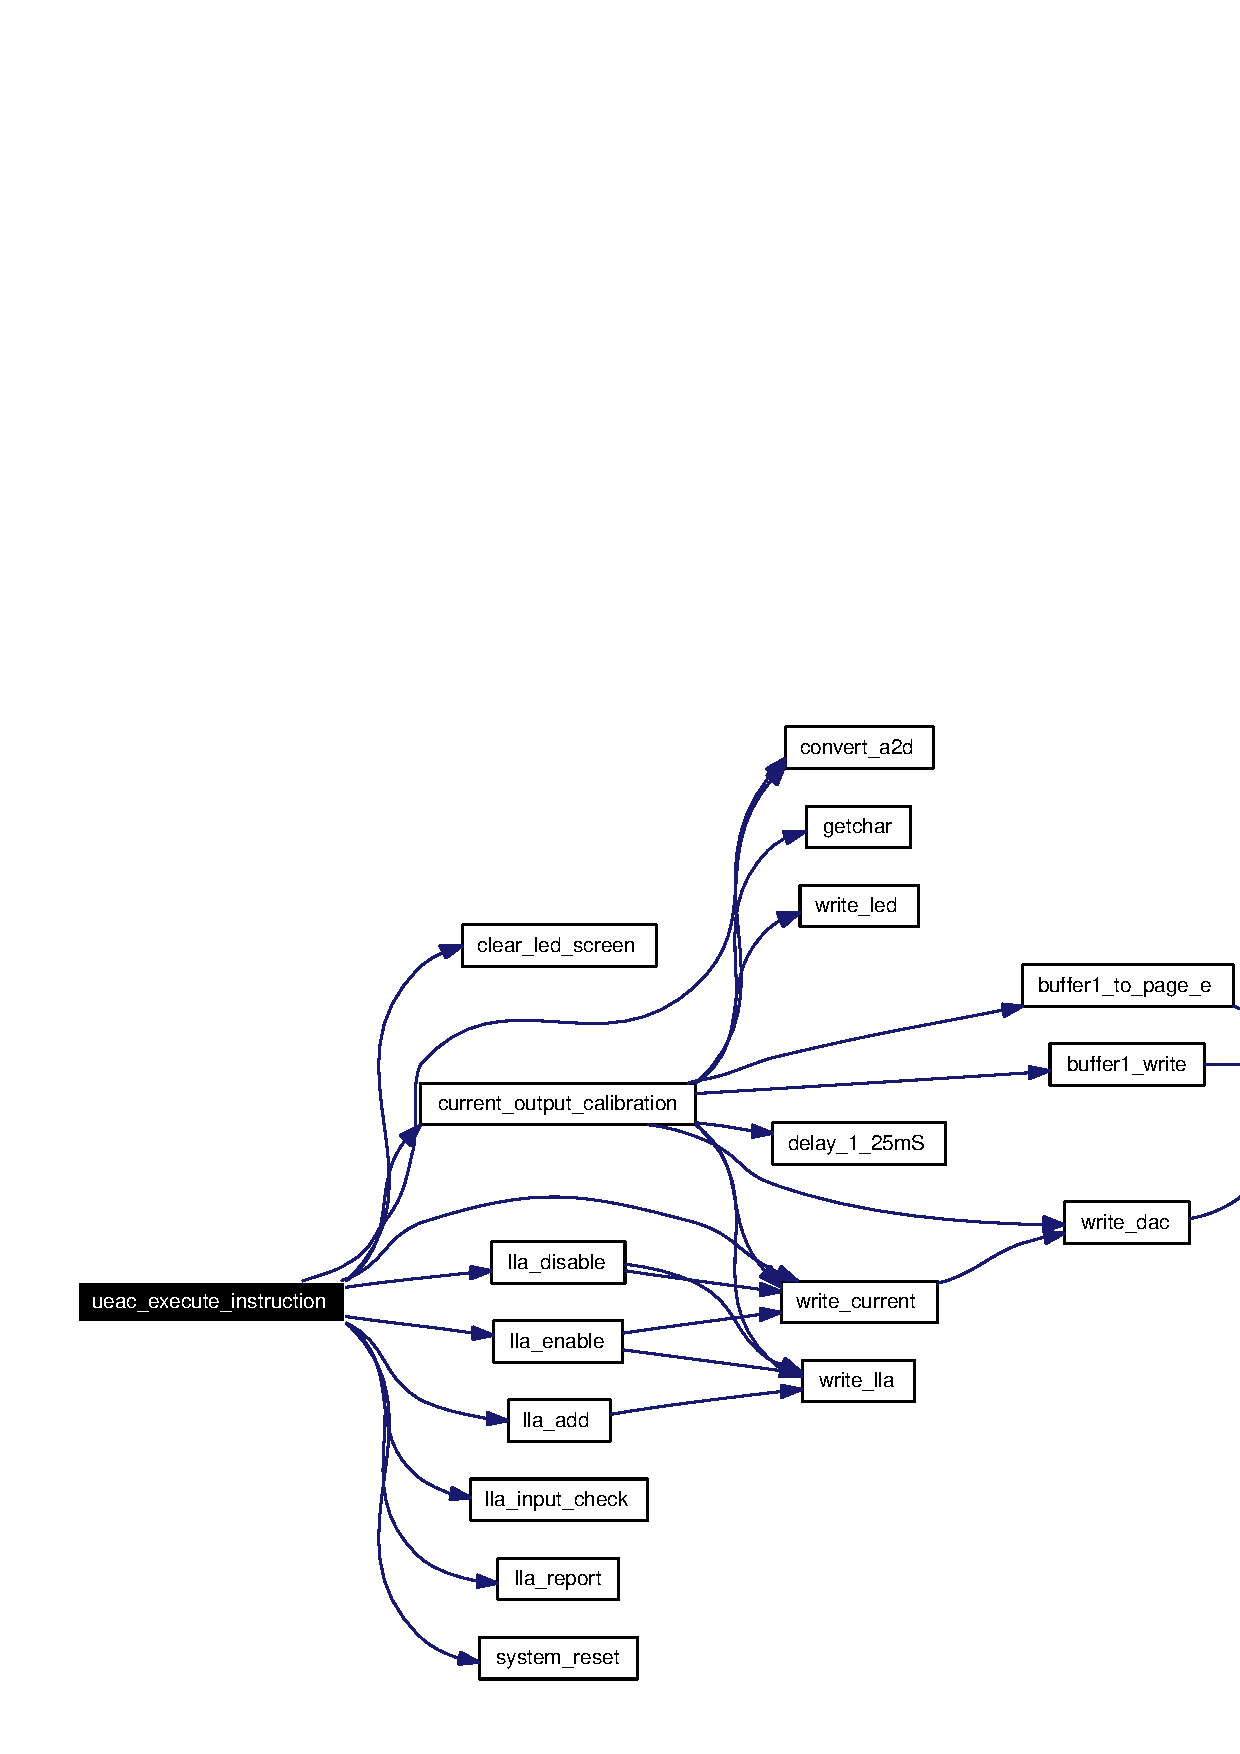
\includegraphics[width=355pt]{ueac_8c_a3_cgraph}
\end{center}
\end{figure}


\subsection{Variable Documentation}
\index{ueac.c@{ueac.c}!lla_data@{lla\_\-data}}
\index{lla_data@{lla\_\-data}!ueac.c@{ueac.c}}
\subsubsection{\setlength{\rightskip}{0pt plus 5cm}{\bf lla\_\-data\_\-t} {\bf lla\_\-data}}\label{ueac_8c_a0}




Definition at line 62 of file ueac.c.